\chapter{Funzioni computabili e URM}
	
	Apriamo il corso definendo l'idea di algoritmo, mostrando come questo possa essere descritto in maniera precisa usando un computer ideale (Macchina a Registri Illimitati), ponendo le basi per la teoria della computabilità.
	
	\section{Unlimited Register Machine}
	Una \textbf{Unlimited Register Machine} è una macchina teorica costituita da un array \textit{potenzialmente} infinito, costituito da registri $R_1, R_2, \dots$ ciascuno dei quali può contenere un numero naturale a precisione infinita. L'informazione non è infinita, in quanto tutti i registri contengono il valore zero, a meno dei registri usati, i quali sono in un numero finito.
	Lo stato di una URM è contenuto nei suoi registri $\vec{r} \in \mathbb{N}^\infty$. Un algoritmo che cambia lo stato interno della URM è detto \textbf{URM-programma}. 
	Un URM-programma è una sequenza finita di $s$ istruzioni $I_1, I_2, \dots, I_s$. 
	\subsection{Configurazione istantanea}
	È una coppia del tipo $(k, \vec{r}) \in \mathbb{N}^+\times \mathbb{N}^\infty$, dove $k$ si chiama  \textbf{contatore di programma}, e rappresenta l'indice dell'istruzione $I_k$ che sta per essere eseguita, mentre $\vec{r}$ è lo stato. 
	
	
\begin{figure}[tbph]
	\centering
	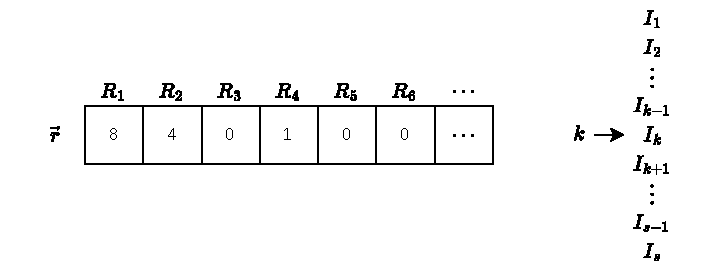
\includegraphics[width=0.7\linewidth]{images/configurazione}
\end{figure}

La configurazione istantanea corrente è $(k, (8,4,0,1,0,0,\dots))$.
	
	\subsection{Istruzioni degli URM-programmi}
	\emph{Un URM-programma è una sequenza finita di $s$ istruzioni $I_1, I_2, \dots, I_s$}. Tra queste, abbiamo:
	\begin{multicols}{2}
	\begin{itemize}
		\item Reset
		\item Incremento
		\item Assegnamento (non necessaria)
		\item Salto condizionato
	\end{itemize}
	\end{multicols}
	
	\paragraph{Istruzione di Reset} $Z(n)$. Azzera il valore contenuto dello slot $n$-esimo. 
	
	$$
	(k, \vec{r}) \xrightarrow{Z(n)} (k+1, \vec{r'}) \quad r_i' = \begin{cases}
	r_i, i \neq n\\
	0, i = n
	\end{cases}
	$$
	
	\paragraph{Istruzione di Incremento} $S(n)$. Incrementa di 1 il valore contenuto dello slot $n$-esimo. 
	
	$$
	(k, \vec{r}) \xrightarrow{S(n)} (k+1, \vec{r'}) \quad r_i' = \begin{cases}
	r_i, i \neq n\\
	r_i +1, i = n \end{cases}
	$$
	
	\paragraph{Istruzione di Assegnamento} $T(m,n)$. Assegna allo slot $n$-esimo il valore contenuto nello slot $m$-esimo. 
	
	$$
	(k, \vec{r}) \xrightarrow{T(m, n)} (k+1, \vec{r'}) \quad r_i' = \begin{cases}
		r_i, i \neq n\\
		r_m, i = n \end{cases}
	$$
	
	\paragraph{Istruzione di Salto condizionato} $J(m,n, q)$. Lo stato rimane lo stesso, ma cambia il contatore di programma $k$.
	
	$$
	(k, \vec{r}) \xrightarrow{J(m, n, q)} (k', \vec{r}) \quad k' = \begin{cases}
		k+1, m \neq n\\
		q, m = n \end{cases}
	$$
	
	
	\section{Definizione di computazione}
	
	Sia $P = \{I_1, I_2, \dots, I_s\}$ un \textbf{programma} con $s$ istruzioni, e $\vec{r}$ lo stato dei registri. La computazione $P(\vec{r})$ di $P$ a partire dallo stato $\vec{r}$ è la sequenza (finita o infinita) di configurazioni istantanee con $k_1 = 1, \vec{r}^{(1)}=\vec{r}$.
	$$
	(k_1, \vec{r}^{(1)}),\;
	(k_2, \vec{r}^{(2)}),\;
	(k_3, \vec{r}^{(3)}),\;
	\ldots,\;
	(k_z, \vec{r}^{(z)}),\;
	(k_{z+1}, \vec{r}^{(z+1)}),\;
	\ldots
	$$
	
	tra queste configurazioni, identifichiamo
	
	\begin{itemize}
		\item Configurazione iniziale, $(1, \vec{r})$.
		\item Configurazione $i$-esima con successore, $(k_i, \vec{r}^{(i)})$. Se $k_i \leq s$, allora ha un successore nella computazione $P(\vec{r})$, e si ha $(k_i, \vec{r}^{(i)}) \xrightarrow{I_{k_{i+1}}} (k_i, \vec{r}^{(i+1)})$
		\item Configurazione finale, $(k_i, \vec{r}^{(i)})$. Se $k_i > s$, allora non ha un successore nella computazione $P(\vec{r})$, e quindi è la \textbf{configurazione finale} della stessa. Si arriva alla configurazione finale tramite esecuzione lineare o salti condizionali.
	\end{itemize}
	
	introduciamo quindi una notazione: $P(\vec{r})$ è un programma con stato iniziale $\vec{r}$,
	$$
	r_i =
	\begin{cases}
		a_i & \text{se } i <n \\
		0 & \text{altrimenti}
	\end{cases}
	$$
	
	$$
	P(a_1, a_2, \ldots, a_n)
	\equiv
	P(a_1, a_2, \ldots, a_n, 0, 0, \ldots)
	$$
	
	In particolare, possiamo indicare se la computazione termina o meno.
	\begin{itemize}
		\item $P(\vec{r})\downarrow$ è una computazione \textbf{terminante};
		\item $P(\vec{r})\uparrow$ è una computazione \textbf{non terminante}
	\end{itemize}
	
	Solitamente, il registro $R_1$ viene usato per l'input e l'output della computazione. Nella notazione, scriveremo che la computazione che torna $b$, $P(\vec{r})\downarrow b$. 
	
	
	\section{Funzione parziale}
	Definiamo $f: A \to B$ funzione parziale, tale che $\text{Dom}(f) \subseteq A$, per cui il dominio potrebbe non essere tutto $A$. Per $a \in A$, se $f$ è definita su $a$, $f(a)\downarrow$, altrimenti $f(a)\uparrow$.
	
	Se $f,g : A \to B$ funzioni parziali, diremo che $f \simeq g$ se:
	\begin{enumerate}
		\item $\forall a \in A: \ f(a)\downarrow \Leftrightarrow g(a)\downarrow$
		\item $\forall a \in A: \ f(a)\downarrow \implies f(a) = g(a) $
	\end{enumerate}
	
	con questa notazione che riprende la terminazione (o non terminazione) dei programmi URM, possiamo indicare se una funzione è definita per un determinato valore dell'insieme $A$.
	
	
	\subsection{Funzioni URM-calcolabili}
	Sia $P$ un programma. $\forall n \geq 1$, poniamo
	$$
	f_P^{(n)}(a_1, a_2, \ldots, a_n) =
	\begin{cases}
		b & \text{se } P(a_1, a_2, \ldots, a_n) \downarrow b \\[6pt]
		\uparrow & \text{se } P(a_1, a_2, \ldots, a_n) \uparrow
	\end{cases}
	$$
	
	chiameremo la funzione parziale $f_P^{(n)} : \mathbb{N}^n \to \mathbb{N}$ la funzione $n$-aria calcolata dal programma $P$.
	Una funzione parziale $g$ si dirà \textbf{URM-calcolabile} se esiste un programma URM $P$ tale che $g \simeq f_P^{(n)}$.

	\paragraph{L'insieme $\mathcal{C}^\text{URM}$ e $\mathcal{C}_n^\text{URM}$}
	La collezione di tutte le funzioni URM-calcolabili  di qualunque arietà si indica con $\mathcal C^\text{URM}$. La collezione di tutte le funzioni URM calcolabili $n$-arie si indica con $\mathcal C_n^\text{URM}$. Scopriremo poi, con la congettura di Church-Turing, che $\mathcal C^\text{URM} = \mathcal C$.
	
	\paragraph{$\mathcal{C}$ è enumerabile} Dimostriamo ciò osservando che $\mathcal{C} = \bigcup_{n=1}^\infty \mathcal C_n^\text{URM}$, e che ciascuna delle $\mathcal C_n$ è costituita da istruzioni del tipo $S(n), Z(n), T(m,n), J(m,n,q)$, che sono enumerabili. Questo vuol dire che il dominio di $\mathcal C^\text{URM}$ è enumerabile, meno denso dell'insieme di tutte le funzioni $f$. 
	
	\section{Esercizi}
	Si allega interprete di programmi-URM online col quale verificare le proprie soluzioni: \url{https://sites.oxy.edu/rnaimi/home/URMsim.htm}
	\subsection{Programmi URM}
	Si dimostri che le seguenti funzioni sono calcolabili esibendo opportuni programmi URM.
	
\subsubsection{Funzione segno}
$$
f(x) = \begin{cases}
	0 & \text{se } x=0\\
	1 & \text{se } x\neq 0
\end{cases}
$$

\begin{algorithm}[H]
	\caption{Funzione segno}
	\begin{algorithmic}[1]
		\State $J(1,2,4)$
		\State $S(2)$
		\State $T(2,1)$
	\end{algorithmic}
\end{algorithm}

\subsubsection{Funzione costante}
$$
f(x) = 5
$$

\begin{algorithm}[H]
	\caption{Funzione costante}
	\begin{algorithmic}[1]
		\State $Z(1)$
		\State $S(1)$
		\State $S(1)$
		\State $S(1)$
		\State $S(1)$
		\State $S(1)$
	\end{algorithmic}
\end{algorithm}

\subsubsection{Funzione uguaglianza}
$$
f(x, y) = \begin{cases}
	0 & \text{se } x=y\\
	1 & \text{se } x\neq y
\end{cases}
$$

\begin{algorithm}[H]
	\caption{Funzione uguaglianza}
	\begin{algorithmic}[1]
		\State $T(1,3)$
		\State $J(2,3,5)$
		\State $Z(1)$
		\State $S(1)$
	\end{algorithmic}
\end{algorithm}

\subsubsection{Funzione minore o uguale}
$$
f(x, y) = \begin{cases}
	0 & \text{se } x\leq y\\
	1 & \text{se } x> y
\end{cases}
$$

\begin{algorithm}[H]
	\caption{Funzione minore o uguale}
	\begin{algorithmic}[1]
		\State $T(1,3)$
		\State $Z(1)$
		\State $S(2)$
		\State $S(4)$
		\State $J(2,4,8)$
		\State $J(3,4,9)$
		\State $J(1,1,4)$
		\State $S(1)$
	\end{algorithmic}
\end{algorithm}

\subsubsection{Funzione x/3}
$$
f(x) =
\begin{cases}
	\dfrac{1}{3}x & \text{se } x \text{ è un multiplo di } 3 \\[6pt]
	\uparrow & \text{altrimenti}
\end{cases}
$$

\begin{algorithm}[H]
	\caption{Funzione $x/3$}
	\begin{algorithmic}[1]
		\State $T(1,4)$
		\State $Z(1)$
		\State $S(1)$
		\State $S(5)$
		\State $S(5)$
		\State $S(5)$
		\State $J(4,5,9)$
		\State $J(1,1,3)$
	\end{algorithmic}
\end{algorithm}

\subsubsection{Funzione $\lfloor 2x/3 \rfloor$}
$$
f(x) =
\begin{cases}
	\lfloor\dfrac{2}{3}x\rfloor & \text{se } x \text{ è un multiplo di } 3 \\[6pt]
	\uparrow & \text{altrimenti}
\end{cases}
$$

\begin{algorithm}[H]
	\caption{Funzione $\lfloor 2x/3 \rfloor$}
	\begin{algorithmic}[1]
	\State TODO
	\end{algorithmic}
\end{algorithm}
	\subsection{Dimostrazioni}
	
	\subsubsection{L'istruzione $T$ non è necessaria}
	
	\begin{algorithm}[H]
		\caption{Istruzione $T$}
		\begin{algorithmic}[1]
			\State Z(m)
			\State S(m)
			\State J(m,n,1)
		\end{algorithmic}
	\end{algorithm}
	
	\subsubsection{Programma senza istruzioni $J$}
	Sia $P$ un programma URM che non contiene alcuna istruzione del tipo $J(m,n,p)$, si dimostra che esiste $m \in \mathbb{N}$ tale che:
	
	
	\section{Correttezza dei programmi}
	
	\paragraph{Correttezza parziale} Un programma $P$ si dice \textbf{parzialmente corretto} rispetto a date specifiche di input $\alpha$ e di output $\beta$ (note rispettivamente come \textbf{precondizione} e \textbf{postcondizione}) se, per ogni input $\vec{x}$ soddisfacente le specifiche $\alpha$, se l'esecuzione di $P$ su $\vec{x}$ è terminante, allora l'output di $P$ soddisfa le specifiche $\beta$.

	$$
	(\forall \vec{x})(\forall b) [(\alpha(\vec{x}) \land P(\vec{x})\downarrow b) \rightarrow \beta(\vec{x}, b)]
	$$
	
	\paragraph{Correttezza totale} Un programma $P$ si dice totalmente corretto rispetto alle specifiche $\alpha$ e $\beta$ se è parzialmente corretto e vale anche la condizione di terminazione:
	
	$$
	(\forall \vec{x})(\alpha(\vec{x}) \rightarrow P(\vec{x})\downarrow)
	$$
	
	\subsection{Esempio di specifiche}
	\paragraph{Correttezza parziale su funzione sottrazione} $\lambda xy.x-y$. Precondizione: $\alpha(x,y) \equiv x \geq 0 \land y \geq 0$. Postcondizione $\beta(x,y,z) \equiv z = x-y$.
	\paragraph{Correttezza totale su funzione sottrazione} $\lambda xy.x-y$. Precondizione: $\alpha(x,y) \equiv x \geq y \land y \geq 0$. Postcondizione $\beta(x,y,z) \equiv z = x-y$
	
	\subsection{Verifica della correttezza parziale dei programmi di Floyd/Hoare}
	Introduciamo adesso delle metodologie per trovare un'asserzione per cui le condizioni di verifica del programma risultino corrette. Usiamo il seguente programma come esempio:
	$$
	\lambda r_1r_2.(r_1+r_2 )
	$$
	\begin{lstlisting}
J(3,2,5)
S(1)
S(3)
J(1,1,1)
	\end{lstlisting}
	
	\begin{figure}[tbph]
		\centering
		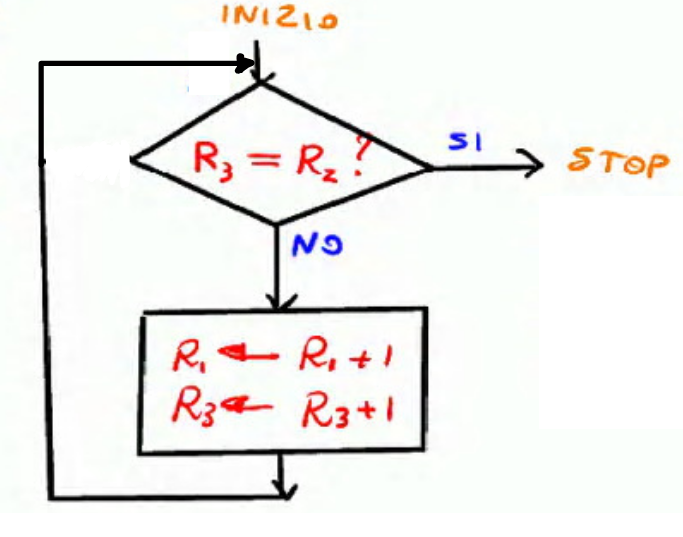
\includegraphics[width=0.5\linewidth]{images/verifica-programma}
	\end{figure}
	
	$$
	precondizione : \begin{cases}
	r_1 = \overline{r_1}\\
	r_2 = \overline{r_2}\\
	r_3 = 0
	\end{cases}
	$$
	
	
	
	\subsection{Verifica della correttezza totale dei programmi}
	Se la verifica della correttezza parziale sfrutta la logica, per la correttezza totale si vuole uno strumento che \textbf{verifica la terminazione} in ogni caso. 
	
	È sufficiente trovare una misura a valori in un insieme ben fondato che decresca strettamente ad ogni iterazione. Possiamo quindi rafforzare l'invariante $A$ con la condizione di decrescita, ottenendo $A^*$. 
	
	\subsection{Sulla verifica della correttezza}
	In generale, metteremo un'asserzione per ogni ciclo condizionale. Il numero di condizioni, invece, è uguale al numero di percorsi.
	
	\section{Predicati}
	Un predicato $n$-ario è una funzione $M : N \to \{true, false\}$. I predicati sono trattati come funzioni, associando ad essi la loro \textbf{funzione caratteristica}.
	
	$$
	c_m(\vec{x}):= \begin{cases}
	1 & \text{se }M(\vec{x})= true\\
	0 & \text{se }M(\vec{x})= false\\
	\end{cases}
	$$
	
	La funzione caratteristica del predicato $x = 0$, ad esempio, è data da
	
	$$
	g(x) = \begin{cases}
	1 & \text{se } x = 0\\
	0 & \text{altrimenti}
	\end{cases}
	$$
	
	\subsection{Predicati decidibili}
	Un predicato si dice \textbf{decidibile} se la sua funzione caratteristica è \textbf{calcolabile}. Scrivere un programma $P$ che calcola la funzione caratteristica è sufficiente per dimostrare che il predicato sia decidibile.
	
	\section{Calcolabilità su altri domini}
	È possibile generalizzare i concetti di decidibilità e calcolabilità ai predicati $M: D \to \{true, false\}$ e funzioni $f : D \to D$ per domini $D \neq \mathbb{N}$: deve esistere tuttavia un modo effettivo per mappare il dominio di $D$ su $\mathbb{N}$.
	
	$$\mathbb{N} \xrightarrow{\alpha^{-1}} D \xrightarrow{f} D \xrightarrow{\alpha} \mathbb{N}$$
	
	Si richiede una codifica effettiva di $D: \alpha: D \to \mathbb{N}$ che sia
	\begin{itemize}
		\item Iniettiva;
		\item Suriettiva;
		\item Effettivamente\footnote{Per effettivo, intendiamo che deve esistere un modo di calcolare la mappatura e l'inversione, un algoritmo vero e proprio.} calcolabile e invertibile.
	\end{itemize}
	
	Definiamo quindi una funzione $f^* = \alpha (f(\alpha^{-1}(x)))$. Questa funzione è calcolabile.
	Un esempio di codifica effettiva per lavorare in $\mathbb{Z}$ è
	
	$$
	\alpha(x) = \begin{cases}
	2x & \text{se } x \geq 0\\
	-2x -1 & \text{altrimenti}
	\end{cases},
	\qquad
	\alpha^{-1}(y) = \begin{cases}
		\dfrac{1}{2}y & \text{se } y \text{ è pari}\\
		-\dfrac{1}{2}(y+1) & \text{altrimenti}
	\end{cases}
	$$
